\subsection{Processo di diffusione in avanti}

Il processo di diffusione in avanti (\emph{forward diffusion process}) è definito come una \emph{catena markoviana} (si veda~\ref{ssec:markov_chain})
che va a perturbare la distribuzione originale, incognita, $q(\mathbf{x}_0)$ di un'immagine $\mathbf{x}_0$ del dataset di addestramento, 
corrompendola con rumore additivo gaussiano (Figura~\ref{fig:forward_diff_process}).

Qualora il suddetto rumore additivo abbia entità contenuta, le \emph{transizioni} della catena markoviana nel processo di diffusione in avanti possono essere 
modellate come distribuzioni gaussiane condizionate (Ho et al., $2020$~\cite{ho2020}). Avvalendosi del formalismo matematico risulta che:
\smallskip
\begin{Mybox1}
\begin{align}
  q(\mathbf{x}_{1:T}|\mathbf{x}_0)  & \triangleq \prod\limits_{t=1}^{T}q(\mathbf{x}_t|\mathbf{x}_{t-1})\quad\quad \text{Processo di diffusione in avanti} \label{eq:forward_process}\\
  q(\mathbf{x}_t | \mathbf{x}_{t-1}) & \triangleq \mathcal{N}(\mathbf{x}_t; \sqrt{1-\beta_t}\mathbf{x}_{t-1},\beta_t \bm{I}) \quad\quad  \text{Generica transizione}\label{eq:forward_chain_transition}
\end{align}
\end{Mybox1}
\smallskip
\noindent dove
\begin{itemize}
  \item $t\in[1,\dots,T]$ è il generico passo temporale.
  \item $\{\beta_t \in (0,1)\}_{t=1}^T$ implementano uno \hyperref[sssec:diff_schedules]{\emph{schema di diffusione}}.
  \item $\mathbf{x}_t$ è l'immagine a valle della $t$-esima transizione della diffusione in avanti.
  \item $\mathbf{x}_0$ è l'immagine originale di partenza che, dopo $T$ passi,
  converge a $\mathbf{x}_T$.
\end{itemize}
\bigskip
\noindent La~\eqref{eq:forward_chain_transition}, in virtù dell'\emph{artificio di riparametrizzazione} 
(si veda~\eqref{eq:rep_trick}), è equivalente ad asserire che
\begin{equation}\label{eq:rep_chain_transition}
 \mathbf{x}_t = \sqrt{1-\beta_t}\mathbf{x}_{t-1} + \sqrt{\beta_t}\bm{\epsilon}_{t-1} 
\end{equation}
dove $\bm{\epsilon}_{t-1} \sim \mathcal{N}(\mathbf{0},\bm{I})$.
\begin{oss}
  Si osserva esplicitamente che, nella~\eqref{eq:forward_chain_transition}, $\mathbf{x}_{t-1}$ è \emph{fissato}:
  il vettore  $\sqrt{1-\beta_t}\mathbf{x}_{t-1}$ è, quindi, \emph{deterministico}.
  Pertanto, dalla~\eqref{eq:forward_chain_transition} si evince che l'immagine $\mathbf{x}_t$ è distribuita come 
  una gaussiana condizionata con media $\bm{\mu}_t=\sqrt{1-\beta_t}\mathbf{x}_{t-1}$ e varianza $\bm{\Sigma}_t=\beta_t\bm{I}$.
\end{oss}
\medskip
\noindent Dalla~\eqref{eq:rep_chain_transition} si desume \emph{come} si ottiene l'immagine al passo 
temporale corrente $\mathbf{x}_t$ a partire dall'immagine $\mathbf{x}_{t-1}$ allo stato
precedente: ad una versione scalata di quest'ultima si aggiunge rumore gaussiano scalato.
Avendo l'accortezza di scegliere i $\beta_t$ opportunamente, si perverrà ad un'immagine $\mathbf{x}_T$ che, per $T$ sufficientemente elevato, 
approssima una distribuzione gaussiana standard ed è, pertanto, indistinguibile dal rumore gaussiano puro~\cite{ho2020}.
\begin{figure}
  \centering
  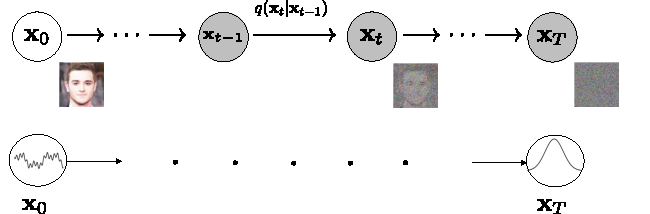
\includegraphics[keepaspectratio]{forward_process2456.pdf} 
  \caption{Processo di diffusione in avanti. Fonte~\cite{ho2020}.} \label{fig:forward_diff_process}
\end{figure}
\medskip
\begin{oss}
Il passaggio dalla~\eqref{eq:forward_chain_transition} alla~\eqref{eq:rep_chain_transition}, ricorrendo all'artificio di 
riparametrizzazione, sarà un \emph{pattern} ricorrente nel prosieguo, in particolare nella riformulazione del processo di diffusione in avanti 
atta a pervenire ad una versione ottimizzata dello stesso.
\end{oss}
\begin{oss}
  Il numero totale degli step di diffusione $T$ è un \emph{iperparametro} e, in quanto tale, 
  va fissato a monte della fase di addestramento del modello. Ho et al.\ ($2020$~\cite{ho2020}) hanno 
  propeso per $T=1000$. 
\end{oss}
\begin{oss}
  È importante osservare che, poiché ad ogni transizione della catena markoviana in avanti viene aggiunto solo del rumore, il
  processo di diffusione in avanti risulta \emph{fissato} qualora si scelgano i $\beta_t$.
\end{oss}
\medskip
\noindent Ricapitolando, il processo di diffusione in avanti trasforma, mediante l'aggiunta progressiva di rumore gaussiano, 
la complessa distribuzione incognita $q(\mathbf{x}_0)$ iniziale in una distribuzione normale standardizzata $\mathcal{N}(\bm{0},\bm{I})$. Il punto 
di forza di una siffatta distribuzione è insito nel suo essere facilmente manipolabile.
La distribuzione terminale della diffusione in avanti costituisce il punto di partenza del processo di diffusione inversa.



\subsubsection{Implementazione del processo di diffusione in avanti}

A beneficio di una maggiore ricchezza argomentativa, nonché per avere un riscontro pratico di 
quanto esposto precedentemente, viene riportata una possibile implementazione del processo di 
diffusione in avanti, partendo da una mia fotografia.

\begin{lstlisting}[language=iPython, caption=Codice adattato da~\cite{nain2022} e implementato con Google Colab~\cite{GoogleColaboratory},label=lst:diff]
import numpy as np                   # per manipolare array e matrici 
from PIL import Image                # per manipolare le immagini  
from matplotlib import pyplot as plt # per creare e visualizzare grafici 
from google.colab import files       # per scaricare l'immagine finale
  
def forward_diff_process(img_t_meno_(*@\color{black}{1}@*), beta, t):
    """
    Tale funzione implementa la generica transizione dall'immagine
    al passo t-1 all'immagine al passo t del processo di diffusione
    in avanti.

    Input:
        img_t_meno_1: immagine al passo precedente (*@$\mathcolor{ipython_red}{(\mathbf{x}_{t-1})}$@*)
        beta: schema di diffusione (vettore di numeri)
        t: passo corrente 
    Output:
        img_t: immagine a valle della transizione (*@$\mathcolor{ipython_red}{(\mathbf{x}_t)}$@*)
    """

    # 1. Si ricava (*@$\mathcolor{ipython_green}{\beta_t}$@*)
    beta_t = beta[t].reshape(-1, 1, 1)  

    # 2. Calcolo media statistica e deviazione standard
    mu = np.sqrt((1.0 - beta_t)) * img_t_meno_(*@\color{black}{1}@*)
    sigma = np.sqrt(beta_t)

    # 3. Generazione dell'immagine al passo t tramite l'equazione(*@\color{ipython_green}{~\eqref{eq:rep_chain_transition}}@*)
    img_t = mu + sigma*np.random.randn(*img_t_meno_(*@\color{black}{1}@*).shape)
    return img_t  

# ------------------------------------------------------------
# Esempio di applicazione del processo di diffusione in avanti  
# ------------------------------------------------------------

# 1. Si carica l'immagine di partenza (*@\color{ipython_green}{$\mathbf{x}_0$}@*)
img = Image.open("../content/selfie.jpg")

# 2. Si ridimensiona l'immagine secondo le dimensioni desiderate
IMG_SIZE = (100, 172)
img = img.resize(size=IMG_SIZE)

# 3. Si definisce il numero dei passi temporali (T)
timesteps = 100

# 4. Implementazione schema di diffusione lineare
beta_start = 0.0001
beta_end = 0.05
beta = np.linspace(beta_start, beta_end, num=timesteps, dtype=np.float(*@\color{black}{32}@*))

immagini_processate = [] 
img_t = np.asarray(img.copy(), dtype=np.float(*@\color{black}{32}@*)) / 255.

# 5.  Esecuzione del processo di diffusione in avanti
#     per ottenere l'immagine a valle di (*@$\mathcolor{ipython_green}{T=100}$@*) passi
for t in range(timesteps):   (*@\label{line:fw_diff}@*)                                                                
    img_t = forward_diff_process(img_t_meno_(*@\color{black}{1}@*)=img_t, beta=beta, t=t)
    if t%20==0 or t==timesteps - 1:   
        immagine = (img_t.clip(0, 1) * 255.0).astype(np.uint(*@\color{black}{8}@*))
        immagini_processate.append(immagine) (*@\label{line:fw_diff1}@*)

# 6. Visualizzazione delle immagini per diversi passi di diffusione
_, ax = plt.subplots(1, len(immagini_processate), figsize=(15, 8))

for i, immagine in enumerate(immagini_processate):
    ax[i].imshow(immagine)
    ax[i].set_title((*@\color{blue}{f}@*)"Timestep: (*@\color{ipython_green}{\{}\color{black}{i}\color{ipython_purple}{*}\color{black}{20}\color{ipython_green}{\}}@*)",fontsize=18)
    ax[i].axis("off")
    ax[i].grid(False)

plt.suptitle("Processo di diffusione in avanti", fontsize=22, y=0.78)
plt.savefig("forward_diff.pdf",pad_inches=0,bbox_inches='tight')
files.download('forward_diff.pdf')
plt.show()
plt.close()
\end{lstlisting}
\smallskip
\begin{center}
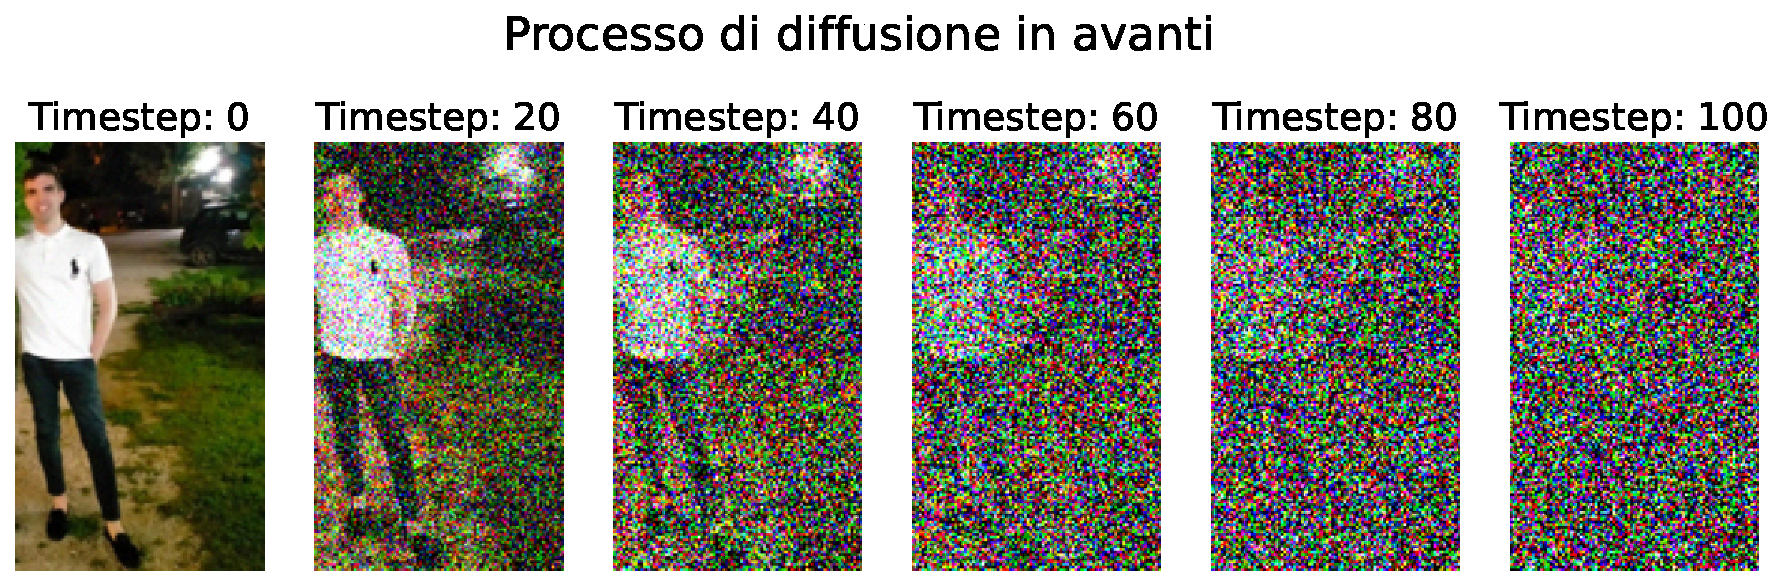
\includegraphics[keepaspectratio, scale=0.4]{code_result.pdf}
\end{center}

\noindent Si noti la progressiva perdita di connotati dell'immagine di partenza che, a valle di 
$T$ passi di diffusione, risulta indistinguibile dal rumore puro. 


%--------------------------------------------------------------

\subsubsection{Ottimizzazione del processo di diffusione in avanti}


Da un'attenta analisi del codice~\ref{lst:diff}, in particolare dalla riga~\ref{line:fw_diff} alla riga~\ref{line:fw_diff1}, si evince 
che, per pervenire all'immagine terminale $\mathbf{x}_T$, è necessario simulare l'\emph{intera} catena markoviana della diffusione in avanti:
all'aumentare del numero di step totali $T$ ciò risulta fortemente inefficiente.
Per ovviare a tale problema, definendo preliminarmente
\begin{equation}
  \alpha_t \triangleq  1-\beta_t, \quad\quad \overline{\alpha}_t  \triangleq \prod\limits_{i=1}^{t}\alpha_i \label{eq:alphas}
\end{equation} 
Ho et al.~\cite{ho2020} hanno osservato che la~\eqref{eq:rep_chain_transition} ammette la seguente riformulazione:
\begin{align}
\mathbf{x}_t & = \sqrt{1-\beta_t}\mathbf{x}_{t-1}+\sqrt{\beta_t}\bm{\epsilon}_{t-1}  \label{eq:eff_forward1}   \\ 
             & = \sqrt{\alpha_t}\mathcolor{blue}{\mathbf{x}_{t-1}}+\sqrt{1-\alpha_t}\bm{\epsilon}_{t-1}  \label{eq:eff_forward2}   \\ 
             & = \sqrt{\alpha_t}\bigl(\mathcolor{blue}{\sqrt{\alpha_{t-1}}\mathbf{x}_{t-2}+\sqrt{1-\alpha_{t-1}}\bm{\epsilon}_{t-2}}\bigr) + \sqrt{1-\alpha_t}\bm{\epsilon}_{t-1} \label{eq:eff_forward3}\\
             & = \sqrt{\alpha_t\alpha_{t-1}}\mathbf{x}_{t-2}+\mathcolor{red}{\sqrt{\alpha_t(1-\alpha_{t-1})}\bm{\epsilon}_{t-2}+\sqrt{1-\alpha_t}\bm{\epsilon}_{t-1}} \label{eq:eff_forward4}\\ 
             & = \sqrt{\alpha_t\alpha_{t-1}}\mathbf{x}_{t-2} + \mathcolor{red}{\sqrt{1-\alpha_t\alpha_{t-1}}\overline{\bm{\epsilon}}_{t-2}} \label{eq:eff_forward5} \\
             & = \dots \\
             & = \sqrt{\alpha_t\alpha_{t-1}\dots\alpha_1}\mathbf{x}_0 + \sqrt{1-\alpha_t\alpha_{t-1}\dots\alpha_1}\bm{\epsilon}_0 \\
             & = \sqrt{\overline{\alpha}_t}\mathbf{x}_0+\sqrt{1-\overline{\alpha}_t}\bm{\epsilon}_0, \label{eq:eff_forward}  
\end{align}

\noindent dove:
\begin{itemize}
  \item $\{\overline{\bm{\epsilon}}_{t},\bm{\epsilon}_{t}\}_{t=0}^T\overset{\text{iid}}{\sim} \mathcal{N}(\bm{0},\bm{I})$.
  \item dalla~\eqref{eq:eff_forward2} alla~\eqref{eq:eff_forward3} ci si è avvalsi dell'artificio di 
        riparametrizzazione~\eqref{eq:rep_trick}.
  \item il passaggio dalla~\eqref{eq:eff_forward4} alla~\eqref{eq:eff_forward5} è il combinato disposto dell'artificio di riparametrizzazione e 
  del risultato per cui una combinazione lineare di vettori gaussiani 
  \emph{indipendenti} è ancora un vettore gaussiano~\eqref{eq:comblingauss_scalar}. Infatti, poiché
  \begin{align}
    \sqrt{1-\alpha_t}\bm{\epsilon_{t-1}} &\sim \mathcal{N}(\bm{0},(1-\alpha_t)\bm{I}) \label{eq:rep_trick1}\\
    \sqrt{\alpha_t(1-\alpha_{t-1})}\bm{\epsilon_{t-2}} &\sim \mathcal{N}(\bm{0},(\alpha_t-\alpha_t\alpha_{t-1})\bm{I}) \label{eq:rep_trick2}
  \end{align}
  ed essendo $\bm{\epsilon_{t-1}}$ ed $\bm{\epsilon_{t-2}}$ \emph{indipendenti}, la somma di~\eqref{eq:rep_trick1} e~\eqref{eq:rep_trick2} è distribuita come
  \[
    \mathcal{N}(\bm{0},(1-\alpha_t+\alpha_t-\alpha_t\alpha_{t-1})\bm{I})=\mathcal{N}(\bm{0},(1-\alpha_t\alpha_{t-1})\bm{I})
  \]
  il che, ricorrendo all'artificio di riparametrizzazione, equivale a:
  \[
    \sqrt{1-\alpha_t}\bm{\epsilon_{t-1}} + \sqrt{\alpha_t(1-\alpha_{t-1})}\bm{\epsilon_{t-2}}
    =\sqrt{1-\alpha_t\alpha_{t-1}}\overline{\bm{\epsilon}}_{t-2}
  \]
\end{itemize} 

\begin{figure}
  \centering
  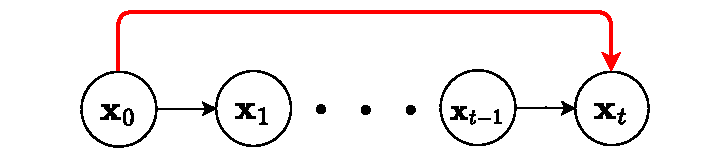
\includegraphics[keepaspectratio, scale=0.8]{forward_process3.pdf}
  \caption{Passaggio diretto da $\mathbf{x}_0$ a $\mathbf{x}_t$. Fonte:~\cite{vaibhavsinghInDepthGuideDenoising2023}.}
 \label{fig:skip_steps}
\end{figure}

\noindent Pertanto, il processo di diffusione in avanti può essere così riformulato:
\begin{Mybox}
\begin{equation}
  q(\mathbf{x}_t|\mathbf{x}_0)=\mathcal{N}\bigl(\mathbf{x}_t;\sqrt{\overline{\alpha}_t}\mathbf{x}_0,(1-\overline{\alpha}_t)\bm{I}\bigr) \label{eq:forward_diff_v2}
\end{equation}
\end{Mybox}
\smallskip
\noindent La riformulazione~\eqref{eq:forward_diff_v2} del processo di diffusione in avanti, basata 
essenzialmente sull'applicazione ricorsiva dell'artificio di riparametrizzazione, apporta un duplice beneficio:
\begin{itemize}
\item dall'immagine di partenza $\mathbf{x}_0$ è possibile raggiungere un $\mathbf{x}_t$ \emph{qualsiasi} con un \emph{unico} step di diffusione in avanti (Figura~\ref{fig:skip_steps}).
\item per progettare uno \emph{schema di diffusione} è possibile avvalersi degli $\overline{\alpha}_t$, in luogo dei $\beta_t$ originali. Il vantaggio di ciò 
risiede nell'interpretazione di $\overline{\alpha}_t$ come la varianza del segnale (l'immagine di partenza $\mathbf{x}_0$) e 
$1-\overline{\alpha}_t$ come la varianza del rumore $\bm{\epsilon}$~\cite{fosterGenerativeDeepLearning2023}.
\end{itemize} 

\noindent Si riporta di seguito l'implementazione della versione ottimizzata del processo di diffusione in avanti, 
per corroborare la perfetta equivalenza sussistente tra le due formulazioni dello stesso, precedentemente investigate.


\begin{lstlisting}[language=iPython,caption=Diffusione in avanti ottimizzata. Codice adattato da~\cite{nain2022},label=lst:diff_ott]
import numpy as np                 
from PIL import Image             
from matplotlib   import pyplot as plt   
from google.colab import files     
    
def forward_diff_process_ott(img_orig, alpha_bar, t):
    """
    Input:
        img_orig: immagine al passo t=0 (*@$(\mathcolor{ipython_red}{\mathbf{x}_0})$@*)
        alpha_bar: versione riparametrizzata di beta
        t: passo corrente 
    Output:
        img_t: immagine ottenuta al passo corrente (*@$(\mathcolor{ipython_red}{\mathbf{x}_t})$@*)
    """
    
    # 1. Si ricava (*@$\mathcolor{ipython_green}{\overline{\alpha}_t}$@*)
    alpha_bar_t = alpha_bar[t].reshape(-1, 1, 1)
    
    # 2. Calcolo media statistica e deviazione standard
    mu = np.sqrt(alpha_bar_t) * img_orig
    sigma = np.sqrt(1.0 - alpha_bar_t)
    
    # 3. Generazione dell'immagine al passo t tramite l'equazione(*@\color{ipython_green}{~\eqref{eq:eff_forward}}@*)
    img_t = mu + sigma * np.random.randn(*img_orig.shape)
    return img_t
  

# 1. Si carica l'immagine di partenza (x0) 
img = Image.open("../content/selfie.jpg")
  
# 2. Si ridimensiona l'immagine secondo le dimensioni desiderate
IMG_SIZE = (100, 172)
img = img.resize(size=IMG_SIZE)
  
# 3. Si definisce il numero dei passi temporali (T)
timesteps = 100

#----------------------------------------------------------
# Versione ottimizzata del processo di diffusione in avanti  
#----------------------------------------------------------

# 4. Implementazione schema di diffusione lineare
beta_start = 0.0001
beta_end = 0.05
beta = np.linspace(beta_start, beta_end, num=timesteps, dtype=np.float32)

# 5. Si definiscono alpha e alpha_bar secondo la (*@\color{ipython_green}{\eqref{eq:alphas}}@*)
alpha = 1.0 - beta
alpha_bar = np.cumprod(alpha)
  
immagini_processate = [img] # immagine (*@$\mathcolor{ipython_green}{\mathbf{x}_0}$@*)
img_orig = np.asarray(img.copy(), dtype=np.float32) / 255.

# 6. Esecuzione del passo di diffusione in avanti per timestep specifici
# Si scelgono gli stessi timestep visualizzati nel codice (*@\color{ipython_green}{\ref{lst:diff}}@*)
timestep_specifici = [19, 39, 59, 79, 99]
for step in timestep_specifici:
    img_t = forward_diff_process_ott(img_orig, alpha_bar, step)
    img_t = (img_t.clip(0, 1) * 255.0).astype(np.uint8)
    immagini_processate.append(img_t)
  

# 7. Visualizzazione delle immagini in diversi passi di diffusione
_, ax = plt.subplots(1, len(immagini_processate), figsize=(15, 8))

for i, sample in enumerate(immagini_processate):
    ax[i].imshow(sample)
    ax[i].set_title((*@\color{blue}{f}@*)"Timestep: (*@\color{ipython_green}{\{}\color{black}{i}\color{ipython_purple}{*}\color{black}{20}\color{ipython_green}{\}}@*)",fontsize=18)
    ax[i].axis("off")
    ax[i].grid(False)

plt.suptitle("Diffusione in avanti ottimizzata",fontsize=22, y=0.78)
plt.savefig("forward_process_v2.pdf",pad_inches=0,bbox_inches='tight')
files.download('forward_process_v2.pdf')
plt.show()
plt.close()
\end{lstlisting}
\begin{center}
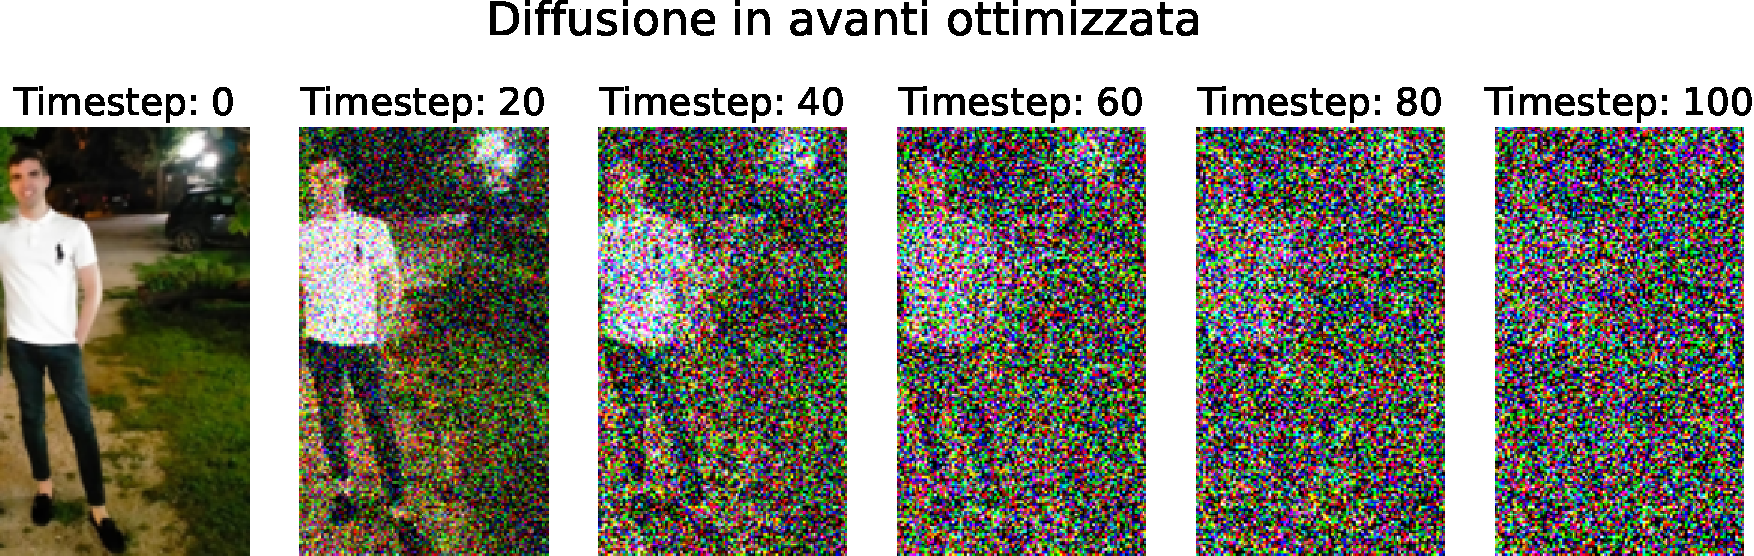
\includegraphics[keepaspectratio, scale=0.4]{efficient_forward_process.pdf}
\end{center}
Si noti che, sebbene il risultato del codice~\ref{lst:diff_ott} sia il medesimo del codice~\ref{lst:diff}, il discrimine tra i due è 
insito nel \emph{modo} in cui si perviene alle immagini nei diversi passi di diffusione.

%---------------------------------------------------------------------
\subsubsection{Schemi di diffusione}\label{sssec:diff_schedules}

\begin{figure}
  \centering
  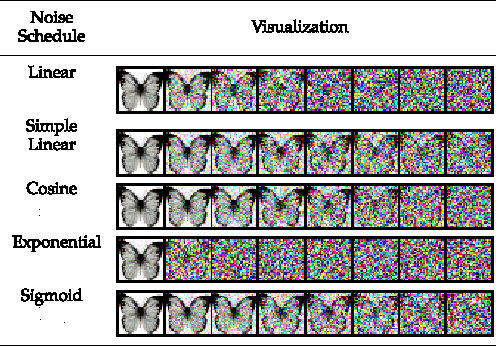
\includegraphics[keepaspectratio, scale=0.9]{diff_schedules}
  \caption{Diversi schemi di diffusione. Fonte:~\cite{changDesignFundDiffusion2023}.}
  \label{fig:diff_schedules}
\end{figure}

Uno schema di diffusione si esplica in una particolare istanza del 
vettore\footnote{Abuso di notazione: l'apice $T$ è l'operazione di \emph{trasposizione},
il pedice $T$ è il numero totale degli step di diffusione.} $\bm{\beta}=(\beta_1,\dots,\beta_T)^T$, e controlla la quantità di rumore 
che viene aggiunta ad ogni passo della catena markoviana nel processo di diffusione in avanti.

\bigskip
\noindent In letteratura si ravvisano due approcci:
\begin{itemize}
\item si addestra una rete neurale ad apprendere i $\beta_t$ che, in tal caso, sono considerati alla stregua di 
parametri ordinari della rete.
Perseguendo tale approccio è possibile implementare schemi di diffusione \emph{diversi} per la fase di addestramento 
e la fase di inferenza~\cite{changDesignFundDiffusion2023}.
\item i $\beta_t$ assurgono ad iperparametri e, in quanto tali, sono fissati a priori (\emph{hyperparameter tuning}). In 
tal caso, per progettare i $\beta_t$, in letteratura, si ricorre ad un ampio ventaglio di tecniche \emph{euristiche}~\cite{changDesignFundDiffusion2023}.
\end{itemize}
Ho et al.~\cite{ho2020} hanno optato per quest'ultimo approccio, propendendo per uno schema di diffusione \emph{lineare} 
in cui i $\beta_t$ crescono linearmente da $\beta_1=10^{-4}$ a $\beta_T=0.02$.

Tuttavia, è stato dimostrato (Nichol et al., $2021$~\cite{nicholImprovedDenoisingDiffusion2021a}) 
che l'impiego di uno schema di diffusione sinusoidale implica un incremento delle prestazioni del modello di diffusione.
In Figura~\ref{fig:diff_schedules} sono riportati diversi schemi di diffusione.

Nel progettare uno schema di diffusione non si deve trascurare l'ingrediente fondamentale nel deep learning: i \emph{dati}.
Dal punto di vista della rappresentazione dei dati, la dimensionalità degli stessi e la massima distanza euclidea tra i campioni di addestramento 
sono fattori da contemplare nel design di uno schema di diffusione~\cite{songImprovedTechniquesTraining2020}. Inoltre, uno schema di diffusione deve 
tener conto della complessità e della ridondanza insita nei dati~\cite{chenImportanceNoiseScheduling2023}. Ad esempio, immagini più grandi potrebbero richiedere più 
rumore additivo, a parità di passi di diffusione in avanti, rispetto ad immagini di dimensioni più piccole~\cite{nicholImprovedDenoisingDiffusion2021a}.

Il \emph{tipo di rumore} aggiunto ad ogni passo del processo di diffusione in avanti è un altro iperparametro: Ho et al.~\cite{ho2020} hanno propeso 
per rumore gaussiano $\bm{\epsilon}\sim\mathcal{N}(\bm{0},\bm{I})$. 
